\section{Caso de estudio}
\subsection{Diseño de la investigación}
El presente trabajo ilustra como caso de estudio la aplicación de la metodología ágil en la gestión de un proyecto de desarrollo de un módulo, integrado a un sistema de gestión y evaluación de competencias de una organización ubicada en los Estados Unidos. El trabajo realizado fue propuesto por la organización que brinda el sistema de gestión de competencias, donde el mismo sirve como base al módulo de gestión curricular a desarrollarse.

El caso refleja de manera práctica cómo se ha desenvuelto un proceso de desarrollo ágil en un diálogo con usuarios ubicados en diferentes localidades como parte del sistema de trabajo. En este proyecto los miembros ubicados en forma remota se encargan del diseño de las tareas, aquí llamadas historias de usuario, a realizarse, y de la validación de las características entregadas.

Debido a que los requisitos de la aplicación a desarrollarse se acordó desde un principio que se irían esclareciendo acorde se vayan completando las funcionalidades, se optó por la metodología ágil como técnica de gestión de desarrollo de software, puesto que era el enfoque más adecuado para poder encarar la problemática.

La observación participante de parte del investigador fue un paso inicial para el desarrollo del sistema en un nuevo equipo, donde se identifican y guían las relaciones con los informantes, lo ayuda a observar de manera embebida la organización y dinámica del equipo, y las prioridades de desarrollo. También, lo permite integrarse con los demás miembros del mismo y de esa manera le facilita el proceso de investigación, además de proveerle una cantidad de interrogantes a ser dilucidadas con los participantes\citep{erlandson_doing_1993}.

El primer paso fue adaptarse a los cambios y a la metodología de trabajo del equipo de desarrollo. Dicho equipo se constituyó luego de a una encuesta previa de capacidades de todos los desarrolladores de la empresa, donde cada uno colocó sus conocimientos en herramientas o en partes del sistema de gestión de competencias, para así poder aprovechar las virtudes de cada persona. Acto seguido se procedió al análisis de las herramientas a utilizarse para corroborar que cumplen con las exigencias del sistema a desarrollarse.

Entre algunas técnicas de recolección de información se utilizan las encuestas\citep{robson_real_2011}. Para este sistema un equipo en Estados Unidos utilizó la misma para proporcionar una visión general de los conocimientos generales del equipo de desarrollo.

Como caso de estudio con enfoque HCI\footnote{de sus siglas en inglés, Human-Computer Interaction, que significa en español interacción humano-computador.}, tuvo como meta la comprensión de problemas o situaciones mediante la interacción del ser humano con la computadora. Además, se buscó una documentación descriptiva del sistema y de su proceso de desarrollo, que apunta a la evolución del modelo propuesto durante el diseño de la misma, finalmente, se brinda y analiza evidencia de que la herramienta haya sido utilizada de manera exitosa mediante demostraciones a los usuarios o validaciones por parte del mismo\citep{lazar_research_2010}. 

Por lo tanto, el caso de estudio es con enfoque HCI y utiliza la observación participante como método principal de recolección de información.

\subsection{Dominio de la problemática}
El proyecto objetivo desarrollado utiliza como base una aplicación web AMS\footnote{de sus siglas en inglés, Assessment Management System, que significa en español sistema de gestión de evaluaciones.} que integra un módulo de gestión curricular a la misma. Los AMS son utilizados por las universidades en Estados Unidos para evaluar las competencias adquiridas de los estudiantes durante el proceso de su carrera o grado. También se busca la disponibilidad en dispositivos móviles. Los dispositivos inteligentes que van a poder utilizar la aplicación se definirán durante el proceso de desarrollo de la misma.

En las aplicaciones dirigidas al ambiente educativo, el hecho de utilizar nuevas tecnologías no asegura una mejor UX\footnote{de sus siglas en inglés, User eXperience, que significa en español experiencia de usuario.}, es por eso que utilizaremos durante el desarrollo de la aplicación técnicas de HCI\citep{lazar_research_2010}, encargadas de utilizar los patrones de diseño e interacción a seguir a la hora de construir cada uno de los componentes de la aplicación a ser desarrollada, y posteriormente validarlos.

Un requisito no funcional que forma parte de la infraestructura del caso de estudio es la utilización de la arquitectura SaaS\footnote{de sus siglas en inglés, Software as a Service, que significa en español software como servicio.}, ya que provee servicios bajo un modelo de pagos de suscripción por las diferentes características que la misma ofrece.

Durante el proceso de desarrollo, se definirán épicas a desarrollarse durante el periodo de diseño de la aplicación y las historias de usuario que están contenidas en las mismas, para que el equipo de desarrollo pueda entregar valor de negocio del módulo integrado en iteraciones cortas de dos semanas.

\subsection{Diseño curricular}
Para aquellas personas ajenas al entorno educativo, en específico aquellas que no forman parte del proceso de diseño curricular puede ser un tanto complejo el proceso de creación y revisión de material curricular en las instituciones. En la actualidad, un formulario de creación o revisión de competencias, cursos, y programas debe pasar por una serie de evaluadores que son los encargados de revisar y verificar que los datos sean válidos.

Hoy día el estado de California cuenta con un patrón de definición de cursos y programas donde la misma sirve como guía para el desarrollo de propuestas para material académico de las universidades. Dicho estándar además contiene una taxonomía de programas e indica cuál es el flujo para la revisión de las propuestas, donde todo es establecido en el PCAH\footnote{de sus siglas en inglés, Program and Course Approval Handbook, que significa en español manual de aprobación de cursos y programas.}\citep{brice_w_harris_program_2013}.

El flujo inicia con el profesor o encargado del curso o programa, una vez completado pasa por la mesa de recepción donde se verifica que cumpla con el estándar estatal para luego pasar por la oficina departamental y la oficina del decano para su revisión de contenido. Una vez revisado y con el visto bueno de ambas oficinas pasa por una última revisión por parte de la oficina curricular para ser registrada en los sistemas de gestión curricular.

Es un proceso que se hace con formularios en papel donde el profesor o encargado del curso o programa tiene que completar los campos requeridos para que el estado de California cuente al curso como válido. Dicho proceso tiene varias deficiencias:
\begin{itemize}
	\item La creación o revisión puede tomar meses debido a los formularios que son completados a mano y requieren de revisión de varias oficinas.
	\item Es un flujo de una sola dirección, eso quiere decir que si es que una de las oficinas rechaza el formulario debe volver a iniciar el flujo.
	\item Se puede producir cuellos de botella en los diferentes puntos de revisión.
\end{itemize}

Una vez ya registrado en los sistemas de gestión curricular es accesible de manera pública para el uso de las universidades del estado de California. De esta manera, si una institución académica posee un sistema de gestión de evaluaciones y quiere incluir los cursos o programas válidos para el estado tiene que ingresar los nuevos datos del sistema de gestión curricular uno a uno como se puede apreciar en la Figura \ref{after_creation}.

\begin{figure}[]
\centering
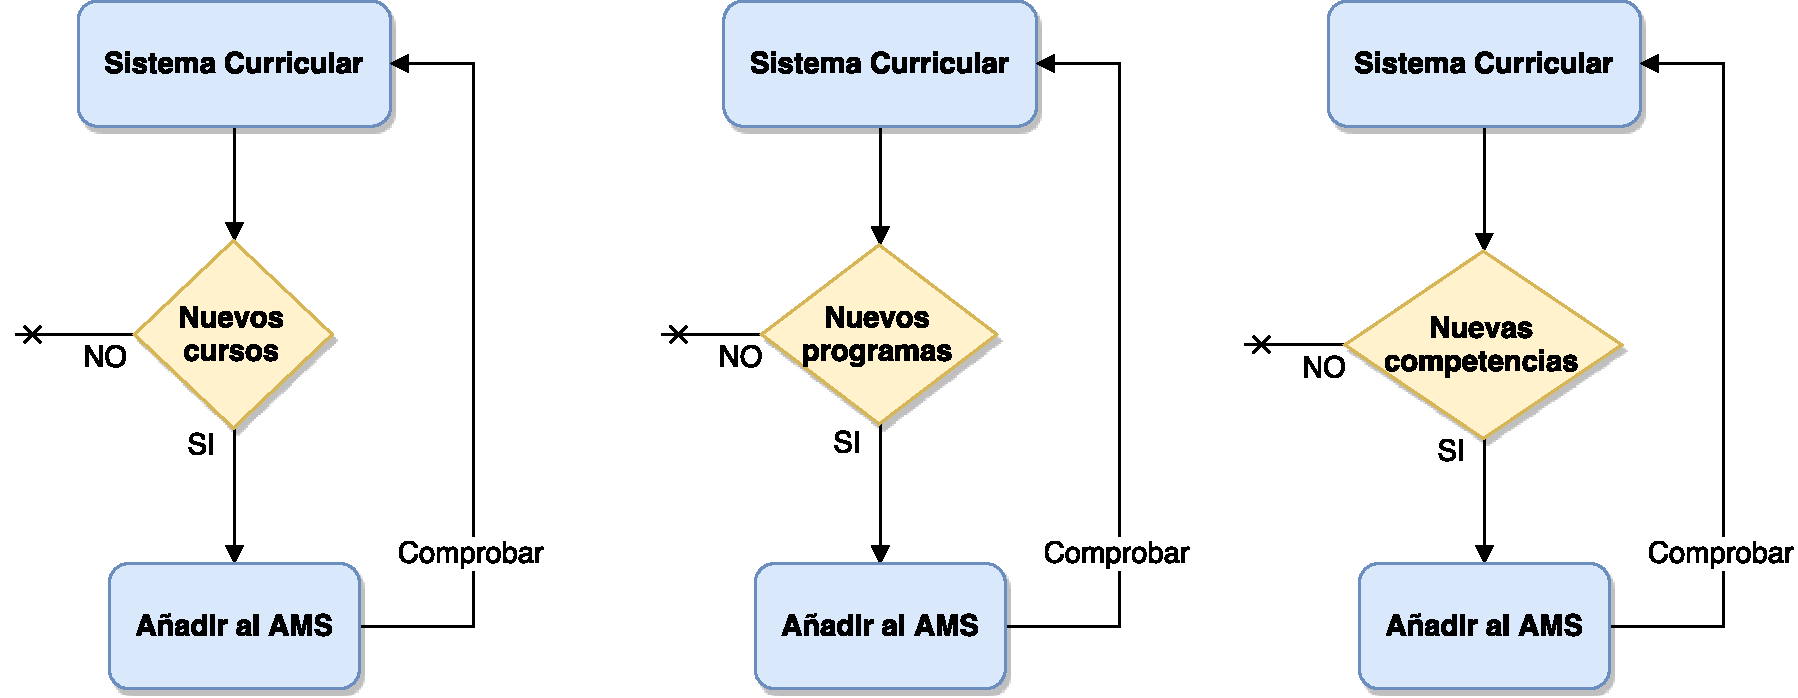
\includegraphics[width=125mm,scale=1]{img/after_creation}
\caption{Proceso de cargar datos desde el sistema curricular al AMS.}
  \label{after_creation}
\end{figure}